\chapter{Kiến trúc Hệ thống Spatial GraphRAG và Khai phá Thực đơn Ngầm}
\label{ch:kien-truc}

\section{Kiến trúc tổng thể 4 tầng của Hệ thống}
\label{sec:ch1-tong-quan}

Để giải quyết đồng bộ các rào cản về ảo giác thực thể, sự bất định vị không gian và sự thiếu hụt dữ liệu đánh giá thực tế, khóa luận đề xuất một kiến trúc hệ thống hoàn chỉnh mang tên Spatial GraphRAG. Hệ thống được tổ chức thành bốn tầng chức năng phân lập và tương tác lỏng lẻo (loosely coupled), bảo đảm khả năng mở rộng quy mô, tính mô-đun hóa cao và thuận tiện trong việc bảo trì, vận hành. Sơ đồ kiến trúc tổng thể bốn tầng của hệ thống được minh họa chi tiết trên Hình \ref{fig:system-architecture}.

\begin{figure}[htbp]
\centering
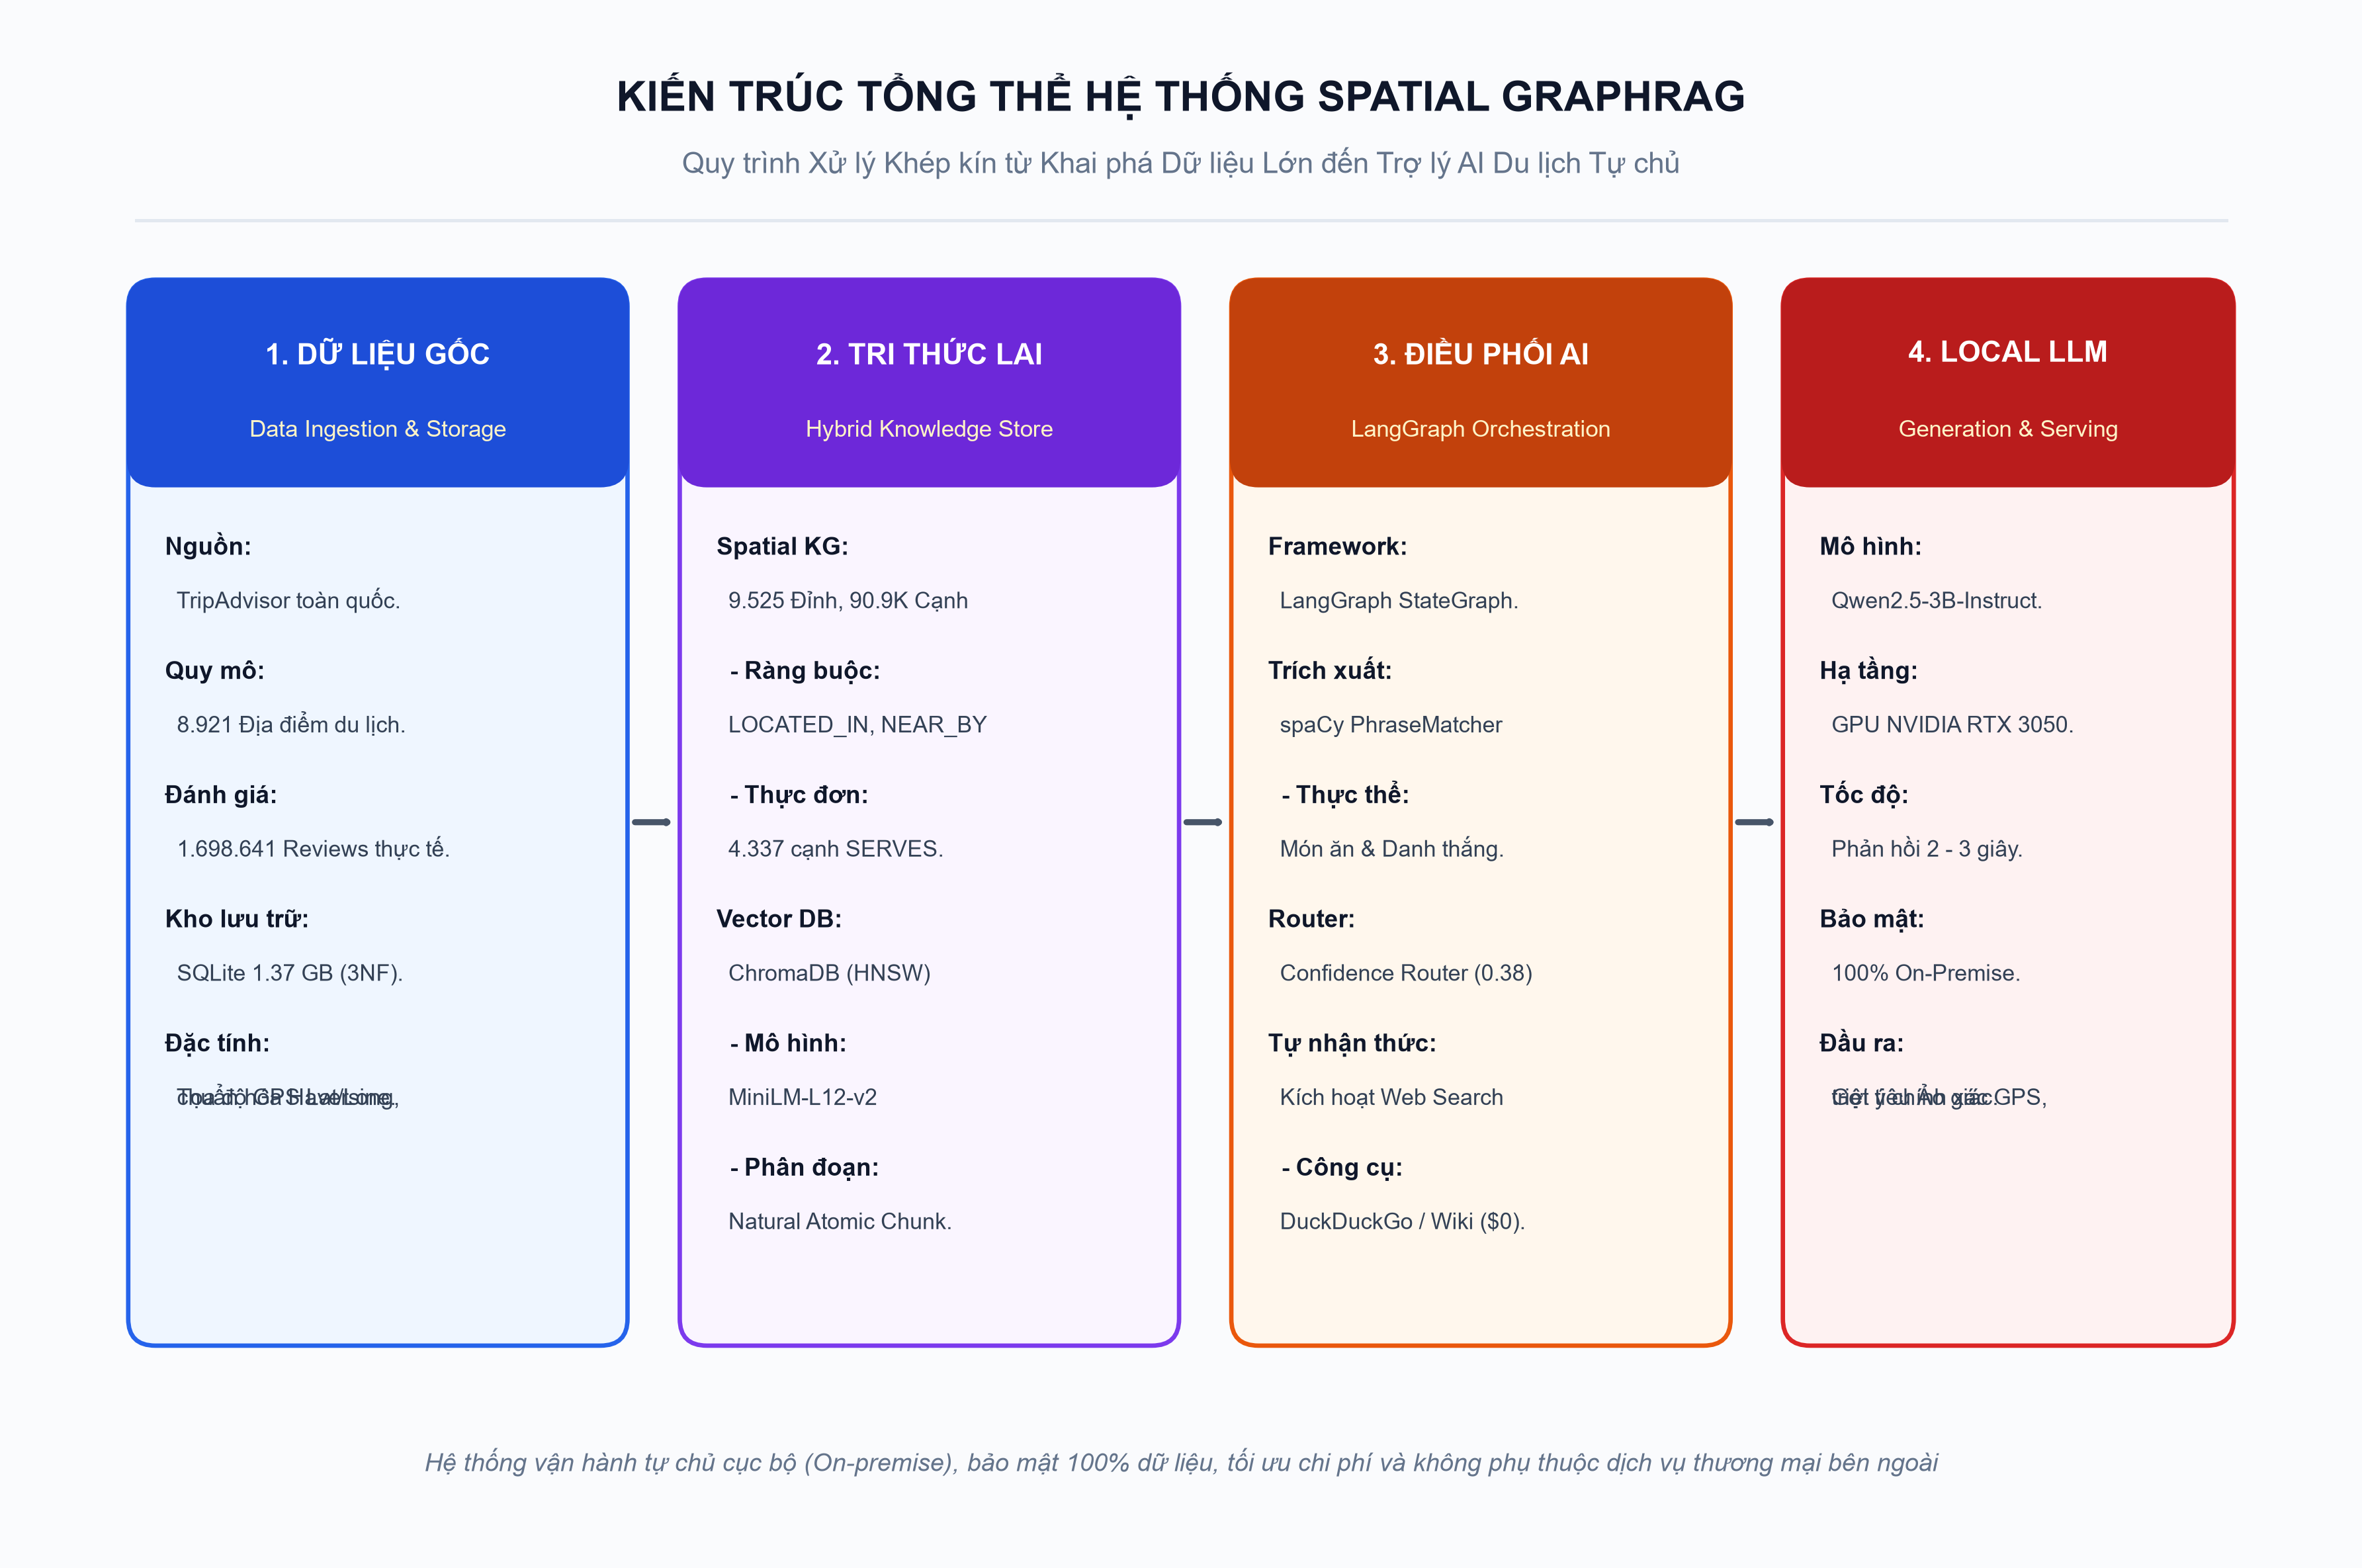
\includegraphics[width=0.92\textwidth]{img/system_architecture.png}
\caption{Kiến trúc tổng thể bốn tầng của Hệ thống Spatial GraphRAG Du lịch Thông minh}
\label{fig:system-architecture}
\end{figure}

Từ sơ đồ tại Hình \ref{fig:system-architecture}, quy trình xử lý luồng dữ liệu và suy luận được vận hành tuần tự qua bốn tầng kiến trúc:

Tầng thứ nhất là Tầng Dữ liệu và Lưu trữ (Data and Storage Layer), chịu trách nhiệm quản lý toàn bộ các nguồn dữ liệu gốc và dữ liệu bán cấu trúc. Tầng này bao gồm cơ sở dữ liệu quan hệ SQLite lưu trữ 1,69 triệu bài nhận xét và hồ sơ thông tin chi tiết của 9.525 địa điểm du lịch; cơ sở dữ liệu vector ChromaDB lưu trữ các véc-tơ nhúng ngữ nghĩa của các phân mảnh nhận xét phân tử; và cấu trúc Đồ thị Tri thức Không gian được biểu diễn và tối ưu hóa trong bộ nhớ thông qua thư viện NetworkX.

Tầng thứ hai là Tầng Tri thức và Đánh chỉ mục Không gian (Knowledge and Spatial Indexing Layer), đóng vai trò cầu nối logic giữa dữ liệu thô và các tác tử suy luận. Tầng này cung cấp ba cơ chế chỉ mục cốt lõi: chỉ mục cự ly không gian dựa trên công thức mặt cầu Haversine phục vụ truy vấn lân cận nhanh với bán kính $\tau_{\text{spatial}} = 1,5\text{ km}$; chỉ mục quan hệ thực đơn ẩm thực $\text{SERVES}$ liên kết các nhà hàng với danh mục 570 món ăn trong từ điển ẩm thực; và bộ mô hình nhúng ngữ nghĩa \texttt{paraphrase-multilingual-MiniLM-L12-v2} chuyển đổi câu hỏi của du khách thành véc-tơ đặc trưng 384 chiều.

Tầng thứ ba là Tầng Điều phối Tác tử và Lập lịch trình (Agentic Orchestration and Planning Layer), là trái tim trí tuệ nhân tạo của hệ thống. Tầng này tích hợp máy trạng thái hữu hạn LangGraph để kiểm soát luồng hội thoại; bộ chấm điểm tin cậy (Confidence Grading Module) đánh giá mức độ bao phủ của tri thức đồ thị; nhánh rẽ dự phòng tìm kiếm Internet (Web Search Fallback) khi cần bổ sung thông tin sự kiện thời gian thực; mô hình ngôn ngữ lớn cục bộ Qwen2.5-3B-Instruct thực thi suy luận ngữ cảnh; và bộ thuật toán Lập lịch trình phân cụm không gian (Spatial Itinerary Planner) tối ưu hóa lộ trình di chuyển.

Tầng thứ tư là Tầng Ứng dụng và Tích hợp Giao diện (Application and Interface Layer), cung cấp hai phương thức tương tác người dùng: Cổng API RESTful chuẩn mở được xây dựng trên nền tảng FastAPI với tài liệu Swagger UI tự động, trả về dữ liệu định dạng JSON chuẩn hóa kèm mảng tọa độ GPS để sẵn sàng tích hợp trực tiếp vào ứng dụng công dân số di động Hue-S của tỉnh Thừa Thiên Huế; và giao diện Web tương tác trực quan phát triển bằng công nghệ bản đồ số (Folium/Leaflet) hỗ trợ du khách tra cứu và quan sát trực tiếp lộ trình trên bản đồ nhiệt.

\section{Thiết kế Đồ thị Tri thức Không gian Du lịch Huế}
\label{sec:ch1-skg-design}

\subsection{Lược đồ cấu trúc thực thể và quan hệ}
\label{subsec:ch1-schema}

Đồ thị Tri thức Không gian Du lịch Huế được thiết kế dựa trên một lược đồ hình thức chặt chẽ, bảo đảm mô hình hóa đầy đủ các khía cạnh không gian, ngữ nghĩa và dịch vụ của một đô thị di sản. Lược đồ phân cấp thực thể và các mối quan hệ ngữ nghĩa của đồ thị được trực quan hóa trên Hình \ref{fig:spatial-kg-schema}.

\begin{figure}[htbp]
\centering
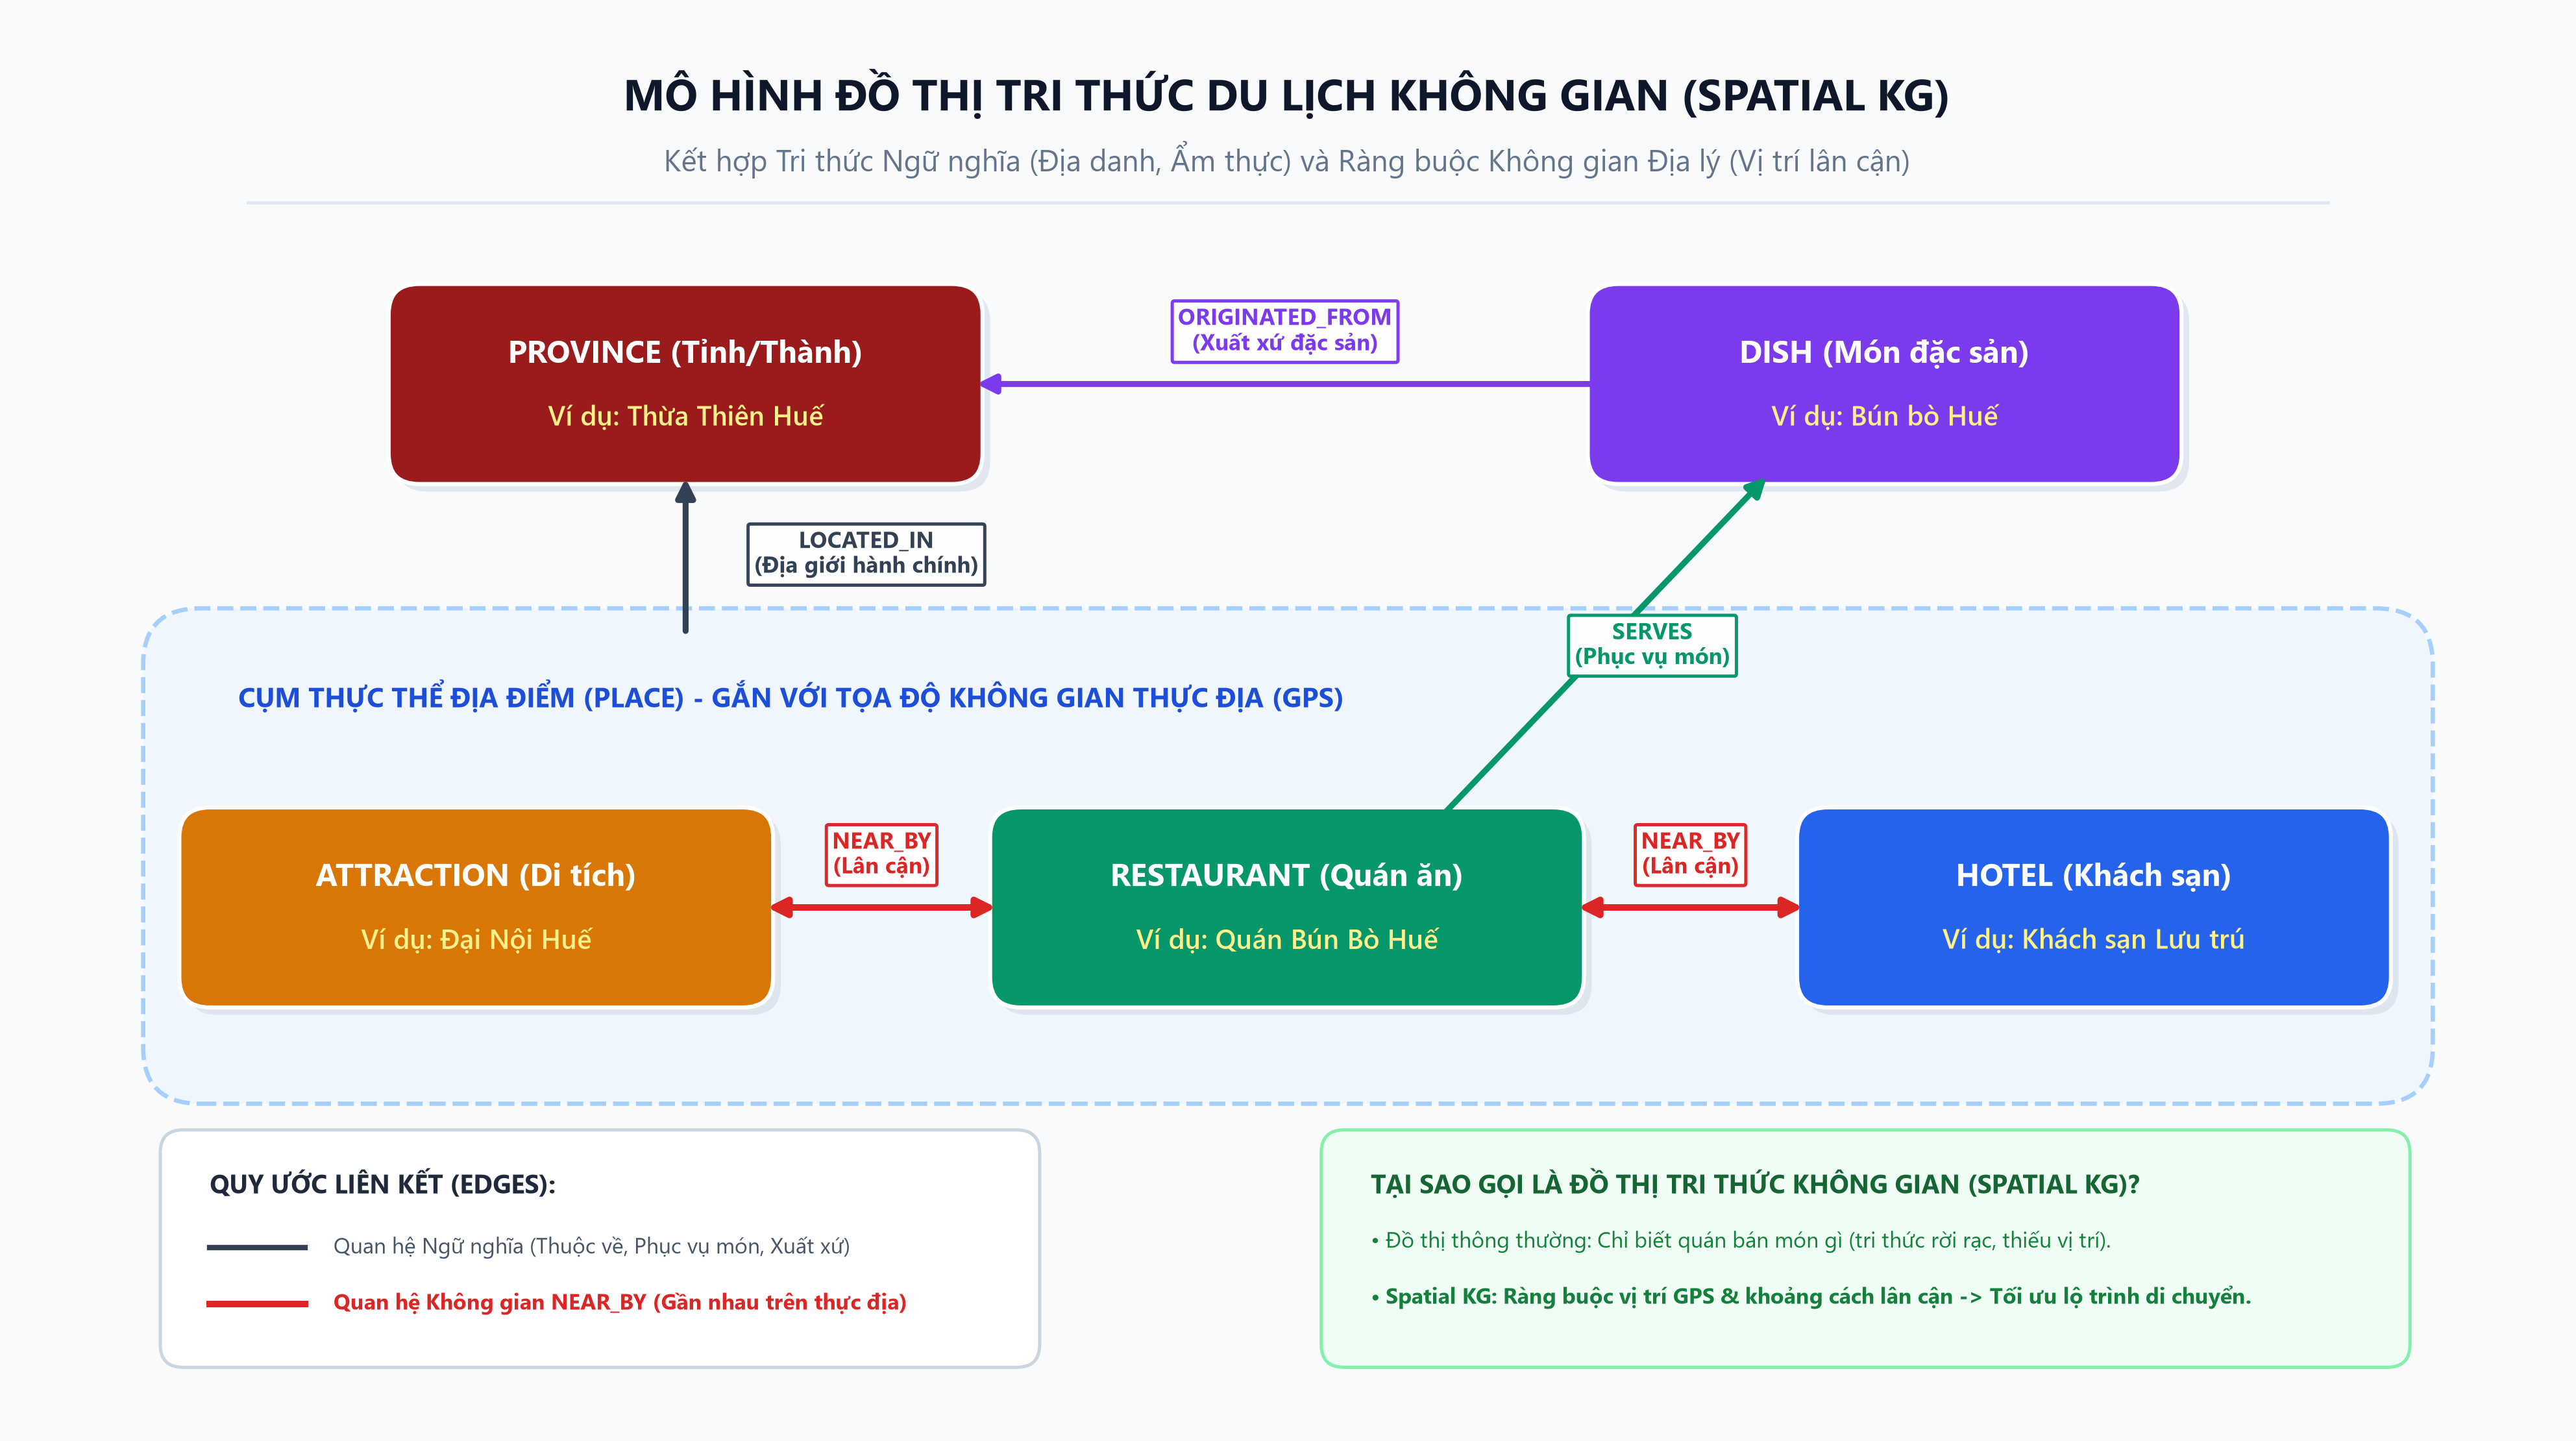
\includegraphics[width=0.88\textwidth]{img/spatial_kg_schema.png}
\caption{Lược đồ cấu trúc thực thể và các mối quan hệ ngữ nghĩa trong Đồ thị Tri thức Không gian}
\label{fig:spatial-kg-schema}
\end{figure}

Theo lược đồ tại Hình \ref{fig:spatial-kg-schema}, hệ thống bao gồm năm lớp nút thực thể chính:
Một là lớp Điểm tham quan (Attraction), đại diện cho các di tích lịch sử, danh lam thắng cảnh, đền chùa, lăng tẩm và bảo tàng tại Huế (như Đại Nội Huế, Chùa Thiên Mụ, Lăng Tự Đức, Đồi Vọng Cảnh, Chợ Đông Ba).
Hai là lớp Cơ sở ẩm thực (Restaurant), bao gồm các nhà hàng, quán ăn truyền thống, quán cà phê và điểm ẩm thực đường phố.
Ba là lớp Cơ sở lưu trú (Hotel), gồm các khách sạn, khu nghỉ dưỡng, nhà nghỉ và homestay.
Bốn là lớp Món ăn đặc sản (Dish), là các thực thể ẩm thực chuẩn hóa thuộc Bộ từ điển ẩm thực Việt Nam (như Bún bò Huế, Cơm hến, Bánh bột lọc, Chè heo quay).
Năm là lớp Khu vực địa lý (Locality), gồm các đơn vị hành chính phường, xã, quận huyện thuộc tỉnh Thừa Thiên Huế và các địa phương phụ cận.

Giữa các lớp thực thể, đồ thị xác lập bốn mối quan hệ ngữ nghĩa cơ bản:
Quan hệ phân cấp địa giới $(u, \text{LOCATED\_IN}, v)$: Kết nối một điểm tham quan hoặc cơ sở dịch vụ $u$ với đơn vị hành chính $v$ chứa nó.
Quan hệ lân cận không gian $(u, \text{NEAR\_BY}, v)$: Được thiết lập tự động giữa hai địa điểm $u$ và $v$ nếu khoảng cách mặt cầu Haversine $d(u, v) \le 1,5\text{ km}$. Cạnh này mang trọng số thực $w = d(u, v)$ phản ánh chính xác cự ly vật lý.
Quan hệ phục vụ ẩm thực $(u, \text{SERVES}, m)$: Kết nối một nhà hàng $u$ với một món ăn đặc sản $m$ nếu món ăn đó được xác nhận thông qua quy trình khai phá dữ liệu nhận xét với điểm tin cậy cao.
Quan hệ phản hồi trải nghiệm $(u, \text{HAS\_REVIEW}, r)$: Kết nối một địa điểm $u$ với các khối văn bản nhận xét phân tử $r$ chứa đựng đánh giá thực tế của du khách.

\subsection{Đặc tính topo và Quy mô dữ liệu đồ thị}
\label{subsec:ch1-topo}

Sau quá trình xử lý và liên kết tự động, đồ thị tri thức đạt quy mô 9.525 nút thực thể và 90.948 cạnh quan hệ. Cấu trúc đồ thị bộc lộ các đặc tính topo mạng lưới điển hình của đồ thị thế giới nhỏ (Small-world Network): các điểm di tích đóng vai trò là các nút trung tâm (hubs) có bậc nút cao, kết nối dày đặc với hàng chục cơ sở ẩm thực và dịch vụ lưu trú xung quanh thông qua các cạnh $\text{NEAR\_BY}$. Bảng \ref{tab:kg-statistics} tổng hợp chi tiết phân bố số lượng nút theo từng lớp thực thể và số lượng cạnh theo từng mối quan hệ.

\begin{table}[htbp]
\centering
\caption{Thống kê định lượng các thành phần trong Đồ thị Tri thức Không gian}
\label{tab:kg-statistics}
\small
\begin{tabularx}{\textwidth}{l r l r}
\hline
\textbf{Lớp thực thể (Entity Type)} & \textbf{Số lượng nút} & \textbf{Loại quan hệ (Relation)} & \textbf{Số lượng cạnh} \\
\hline
Attraction (Điểm tham quan) & 1.842 & NEAR\_BY (Lân cận $\le 1,5\text{ km}$) & 64.218 \\
Restaurant (Ẩm thực, quán ăn) & 4.120 & SERVES (Phục vụ món ăn) & 14.850 \\
Hotel (Lưu trú, khách sạn) & 2.650 & LOCATED\_IN (Thuộc địa phương) & 9.525 \\
Dish (Món ăn đặc sản) & 570 & HAS\_REVIEW (Liên kết nhận xét) & 2.355 \\
Locality (Đơn vị địa lý) & 343 & -- & -- \\
\hline
\textbf{Tổng số nút thực thể} & \textbf{9.525} & \textbf{Tổng số cạnh quan hệ} & \textbf{90.948} \\
\hline
\end{tabularx}
\end{table}

Quy mô định lượng tại Bảng \ref{tab:kg-statistics} chứng minh rằng hơn 70\% số cạnh trong đồ thị là các liên kết không gian $\text{NEAR\_BY}$, phản ánh mật độ kết nối dày đặc giữa các dịch vụ du lịch trong bán kính đi bộ. Cấu trúc mạng lưới này cho phép giải thuật tìm kiếm thực hiện duyệt đồ thị theo chiều sâu hoặc chiều rộng (Graph Traversal) trong thời gian dưới 10 mili-giây, tạo tiền đề để hệ thống lọc sạch các địa điểm ở xa trước khi chuyển ngữ cảnh cho mô hình ngôn ngữ lớn.

\section{Khai phá Thực đơn Ngầm từ Dữ liệu Nhận xét Du khách}
\label{sec:ch1-menu-mining}

Để giải quyết bài toán menu tĩnh và lấp đầy các khoảng trống thông tin về món ăn đặc sản, nghiên cứu ứng dụng quy trình khai phá dữ liệu nhận xét dựa trên Bộ từ điển ẩm thực 570 món ăn. Mỗi bài nhận xét của du khách được quét qua một bộ lọc đối sánh thực thể xâu chuỗi (Aho-Corasick Automaton) kết hợp bộ quy tắc khử nhiễu từ đồng âm (ví dụ: phân biệt giữa từ ``bánh khoái'' chỉ món ăn và tính từ ``khoái chí'', hay ``cơm hến'' và danh từ chỉ loài sinh vật ``hến'').

Mỗi khi phát hiện sự xuất hiện đồng thời của một món ăn đặc sản $m$ trong bài nhận xét viết về cơ sở ăn uống $u$, hệ thống tiến hành bóc tách phân cực cảm xúc của câu văn chứa món ăn đó. Cạnh quan hệ $(u, \text{SERVES}, m)$ chỉ được xác lập chính thức trên đồ thị khi chỉ số tin cậy $\text{Conf}(u, m)$ được định nghĩa trong công thức (\ref{eq:dish-confidence}) vượt qua ngưỡng $\tau_{\text{dish}} = 0,70$ và số lượng bài nhận xét khen ngợi tối thiểu từ 3 du khách độc lập trở lên.

Bảng \ref{tab:mined-dishes-sample} minh họa một số kết quả khai phá thực đơn ngầm tiêu biểu tại các quán ăn truyền thống nổi tiếng ở Huế so sánh với danh mục đăng ký ban đầu.

\begin{table}[htbp]
\centering
\caption{Mẫu đối soát kết quả khai phá thực đơn ngầm từ nhận xét du khách tại Huế}
\label{tab:mined-dishes-sample}
\small
\begin{tabularx}{\textwidth}{l l >{\raggedright\arraybackslash}X c}
\hline
\textbf{Tên quán ăn thực tế} & \textbf{Địa chỉ tại Huế} & \textbf{Món đặc sản khai phá từ Reviews} & \textbf{Số lượt bảo chứng} \\
\hline
Bún bò Mụ Rơi & 40 Nguyễn Chí Diểu & Bún bò giò heo, Chả cua, Gân bò & 342 lượt \\
Bánh bèo Bà Đỏ & 08 Nguyễn Bỉnh Khiêm & Bánh bèo chén, Bánh nậm, Bánh lọc gói & 518 lượt \\
Cơm hến Hoa Đông & 64 kiệt 7 Ưng Bình & Cơm hến, Bún hến, Mì hến, Chè bắp & 412 lượt \\
Quán Hạnh & 11 Phù Đổng Thiên Vương & Bánh khoái, Nem lụi, Cuốn thịt nướng & 685 lượt \\
Chè Hẻm & 01 kiệt 29 Hùng Vương & Chè bột lọc heo quay, Chè hạt sen & 294 lượt \\
\hline
\end{tabularx}
\end{table}

Bảng \ref{tab:mined-dishes-sample} chứng minh rằng quy trình khai phá dữ liệu đã bóc tách chính xác các món ăn cốt lõi làm nên thương hiệu của từng quán. Những thông tin này hoàn toàn không có trong danh bạ phân loại kinh doanh chung (vốn chỉ phân loại chung là ``Nhà hàng Việt Nam''), chứng minh tính đúng đắn của Giả thuyết $H_2$ về khả năng làm giàu tri thức ẩm thực địa phương từ dữ liệu du khách.

\section{Khung điều phối Agentic RAG trên LangGraph}
\label{sec:ch1-langgraph}

\subsection{Máy trạng thái StateGraph và Luồng xử lý đa tác tử}
\label{subsec:ch1-stategraph}

Kiến trúc tác tử thông minh của Spatial GraphRAG được hiện thực hóa dưới dạng một Đồ thị Trạng thái (StateGraph) trên thư viện LangGraph. Sơ đồ luồng điều phối trạng thái và các nhánh rẽ điều kiện được trực quan hóa trên Hình \ref{fig:langgraph-architecture}.

\begin{figure}[htbp]
\centering
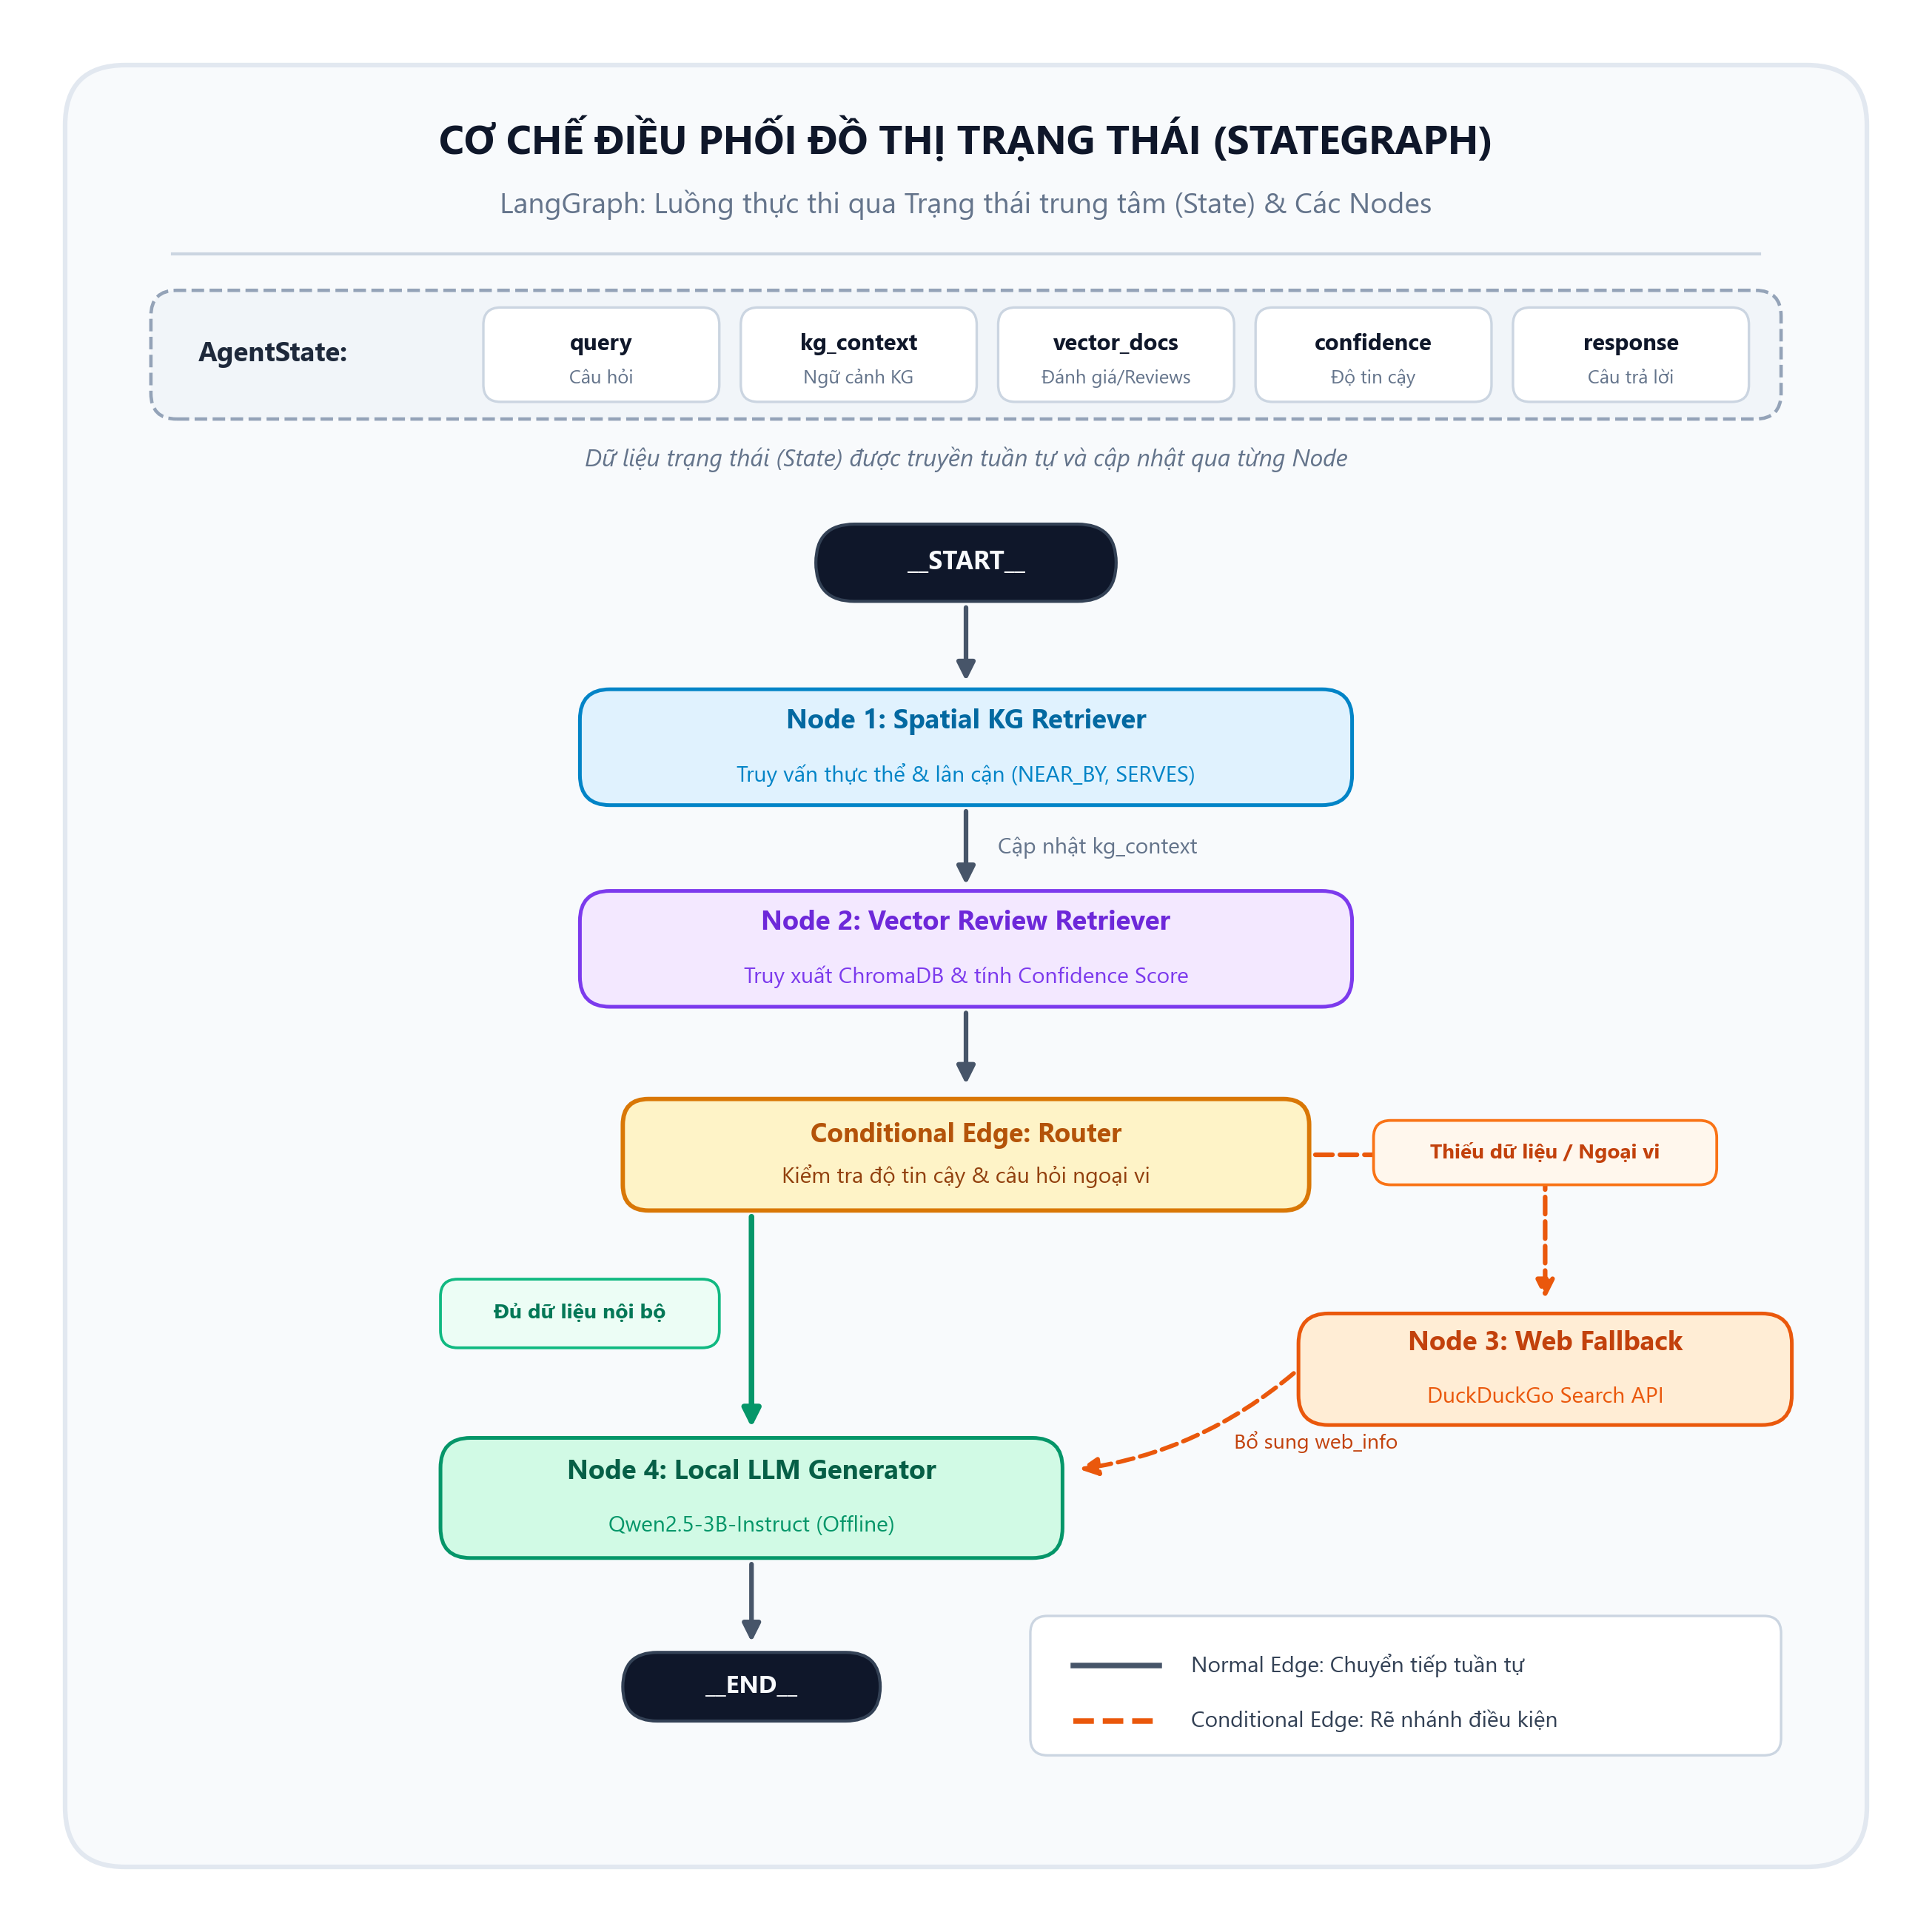
\includegraphics[width=0.95\textwidth]{img/langgraph_architecture.png}
\caption{Kiến trúc Đồ thị Trạng thái (StateGraph) điều phối quy trình Agentic RAG trên LangGraph}
\label{fig:langgraph-architecture}
\end{figure}

Theo kiến trúc minh họa tại Hình \ref{fig:langgraph-architecture}, quy trình xử lý của tác tử trải qua năm nút trạng thái tuần tự và có điều kiện:

Nút 1: Trích xuất ý định và thực thể (Entity and Intent Extraction). Khi nhận câu hỏi từ du khách, nút này sử dụng mô hình Qwen2.5-3B với cấu trúc Prompt ép kiểu JSON để trích xuất các thông tin then chốt: loại truy vấn (hỏi đáp POI đơn lẻ, tìm quán ăn lân cận, hay lập lịch trình nhiều ngày), tên địa danh neo (Anchor POI), món ăn mong muốn, và ngân sách thời gian.

Nút 2: Truy vấn Đồ thị Tri thức Không gian (Spatial Graph Retrieval). Dựa trên Anchor POI đã nhận diện, hệ thống truy xuất các nút láng giềng trên đồ thị NetworkX thông qua các cạnh $\text{NEAR\_BY}$ trong bán kính $d \le 1,5\text{ km}$, đồng thời lọc theo cạnh $\text{SERVES}$ nếu câu hỏi có yêu cầu về món ăn đặc sản. Đồng thời, các phân mảnh nhận xét liên quan từ ChromaDB được truy xuất để bổ sung đánh giá thực tế.

Nút 3: Đánh giá độ tin cậy ngữ cảnh (Confidence Grading Node). Nút này hoạt động như một cơ chế tự suy ngẫm (Self-reflection), tính toán chỉ số tin cậy tổng hợp $S_{\text{conf}}$ dựa trên công thức toán học:
\begin{equation}
    S_{\text{conf}} = \alpha \cdot S_{\text{grounding}} + \beta \cdot (1 - S_{\text{violation}}) + \gamma \cdot S_{\text{dish}}
    \label{eq:confidence-score}
\end{equation}
trong đó $S_{\text{grounding}} \in [0, 1]$ là tỷ lệ các thực thể trong ngữ cảnh có mặt hợp lệ trên đồ thị tri thức; $S_{\text{violation}} \in [0, 1]$ là tỷ lệ các địa điểm bị vi phạm cự ly bán kính $1,5\text{ km}$; $S_{\text{dish}} \in [0, 1]$ là tỷ lệ khớp nối món ăn yêu cầu; và $\alpha, \beta, \gamma$ là các hệ số trọng số thỏa mãn $\alpha + \beta + \gamma = 1$, được nghiên cứu thiết lập thực nghiệm tương ứng là $\alpha = 0,4$, $\beta = 0,3$ và $\gamma = 0,3$.

Nút 4: Phân luồng dự phòng tìm kiếm mạng (Web Search Fallback). Nếu điểm số tin cậy $S_{\text{conf}} < \tau_{\text{conf}} = 0,65$ (xảy ra khi du khách hỏi về các sự kiện thời sự mới phát sinh ngoài phạm vi đồ thị tĩnh), cạnh có điều kiện sẽ kích hoạt nhánh rẽ sang công cụ tìm kiếm DuckDuckGo/Google Search để thu thập các trang tin mới nhất, sau đó hợp nhất vào ngữ cảnh. Ngược lại, nếu $S_{\text{conf}} \ge 0,65$, hệ thống chuyển thẳng sang nút tạo sinh.

Nút 5: Tạo sinh câu trả lời có kiểm soát (Constrained Generation Node). Mô hình Qwen2.5-3B tiếp nhận toàn bộ ngữ cảnh đã được neo giữ (grounded context) từ đồ thị tri thức để sinh câu trả lời bằng tiếng Việt tự nhiên, bảo đảm không bịa đặt bất kỳ thông tin nào ngoài các nút thực thể đã được cung cấp.
